\documentclass[letterpaper,12pt]{cicese}
	\usepackage[letterpaper,left=2.5cm,right=2.5cm,top=3cm,bottom=3cm]{geometry}
	\usepackage{setspace}
	\usepackage{natbib}
	\usepackage{graphicx}
	\usepackage{caption}
	\usepackage{cicese}
	% Macros for Scientific Word 3.0 documents saved with the LaTeX filter.
%Copyright (C) 1994-97 TCI Software Research, Inc.
\typeout{TCILATEX Macros for Scientific Word 3.0 <05 August 1998>.}
\typeout{NOTICE:  This macro file is NOT proprietary and may be 
freely copied and distributed.}
%
\makeatletter
%
%%%%%%%%%%%%%%%%%%%%%%
% macros for time
\newcount\@hour\newcount\@minute\chardef\@x10\chardef\@xv60
\def\tcitime{
\def\@time{%
  \@minute\time\@hour\@minute\divide\@hour\@xv
  \ifnum\@hour<\@x 0\fi\the\@hour:%
  \multiply\@hour\@xv\advance\@minute-\@hour
  \ifnum\@minute<\@x 0\fi\the\@minute
  }}%

%%%%%%%%%%%%%%%%%%%%%%
% macro for hyperref
\@ifundefined{hyperref}{\def\hyperref#1#2#3#4{#2\ref{#4}#3}}{}

% macro for external program call
\@ifundefined{qExtProgCall}{\def\qExtProgCall#1#2#3#4#5#6{\relax}}{}
%%%%%%%%%%%%%%%%%%%%%%
%
% macros for graphics
%
\def\FILENAME#1{#1}%
%
\def\QCTOpt[#1]#2{%
  \def\QCTOptB{#1}
  \def\QCTOptA{#2}
}
\def\QCTNOpt#1{%
  \def\QCTOptA{#1}
  \let\QCTOptB\empty
}
\def\Qct{%
  \@ifnextchar[{%
    \QCTOpt}{\QCTNOpt}
}
\def\QCBOpt[#1]#2{%
  \def\QCBOptB{#1}
  \def\QCBOptA{#2}
}
\def\QCBNOpt#1{%
  \def\QCBOptA{#1}
  \let\QCBOptB\empty
}
\def\Qcb{%
  \@ifnextchar[{%
    \QCBOpt}{\QCBNOpt}
}
\def\PrepCapArgs{%
  \ifx\QCBOptA\empty
    \ifx\QCTOptA\empty
      {}%
    \else
      \ifx\QCTOptB\empty
        {\QCTOptA}%
      \else
        [\QCTOptB]{\QCTOptA}%
      \fi
    \fi
  \else
    \ifx\QCBOptA\empty
      {}%
    \else
      \ifx\QCBOptB\empty
        {\QCBOptA}%
      \else
        [\QCBOptB]{\QCBOptA}%
      \fi
    \fi
  \fi
}
\newcount\GRAPHICSTYPE
%\GRAPHICSTYPE 0 is for TurboTeX
%\GRAPHICSTYPE 1 is for DVIWindo (PostScript)
%%%(removed)%\GRAPHICSTYPE 2 is for psfig (PostScript)
\GRAPHICSTYPE=\z@
\def\GRAPHICSPS#1{%
 \ifcase\GRAPHICSTYPE%\GRAPHICSTYPE=0
   \special{ps: #1}%
 \or%\GRAPHICSTYPE=1
   \special{language "PS", include "#1"}%
%%%\or%\GRAPHICSTYPE=2
%%%  #1%
 \fi
}%
%
\def\GRAPHICSHP#1{\special{include #1}}%
%
% \graffile{ body }                                  %#1
%          { contentswidth (scalar)  }               %#2
%          { contentsheight (scalar) }               %#3
%          { vertical shift when in-line (scalar) }  %#4
\def\graffile#1#2#3#4{%
%%% \ifnum\GRAPHICSTYPE=\tw@
%%%  %Following if using psfig
%%%  \@ifundefined{psfig}{\input psfig.tex}{}%
%%%  \psfig{file=#1, height=#3, width=#2}%
%%% \else
  %Following for all others
  % JCS - added BOXTHEFRAME, see below
    \bgroup
    \leavevmode
    \@ifundefined{bbl@deactivate}{\def~{\string~}}{\activesoff}
    \raise -#4 \BOXTHEFRAME{%
        \hbox to #2{\raise #3\hbox to #2{\null #1\hfil}}}%
    \egroup
}%
%
% A box for drafts
\def\draftbox#1#2#3#4{%
 \leavevmode\raise -#4 \hbox{%
  \frame{\rlap{\protect\tiny #1}\hbox to #2%
   {\vrule height#3 width\z@ depth\z@\hfil}%
  }%
 }%
}%
%
\newcount\draft
\draft=\z@
\let\nographics=\draft
\newif\ifwasdraft
\wasdraftfalse

%  \GRAPHIC{ body }                                  %#1
%          { draft name }                            %#2
%          { contentswidth (scalar)  }               %#3
%          { contentsheight (scalar) }               %#4
%          { vertical shift when in-line (scalar) }  %#5
\def\GRAPHIC#1#2#3#4#5{%
 \ifnum\draft=\@ne\draftbox{#2}{#3}{#4}{#5}%
  \else\graffile{#1}{#3}{#4}{#5}%
  \fi
 }%
%
\def\addtoLaTeXparams#1{%
    \edef\LaTeXparams{\LaTeXparams #1}}%
%
% JCS -  added a switch BoxFrame that can 
% be set by including X in the frame params.
% If set a box is drawn around the frame.

\newif\ifBoxFrame \BoxFramefalse
\newif\ifOverFrame \OverFramefalse
\newif\ifUnderFrame \UnderFramefalse

\def\BOXTHEFRAME#1{%
   \hbox{%
      \ifBoxFrame
         \frame{#1}%
      \else
         {#1}%
      \fi
   }%
}


\def\doFRAMEparams#1{\BoxFramefalse\OverFramefalse\UnderFramefalse\readFRAMEparams#1\end}%
\def\readFRAMEparams#1{%
 \ifx#1\end%
  \let\next=\relax
  \else
  \ifx#1i\dispkind=\z@\fi
  \ifx#1d\dispkind=\@ne\fi
  \ifx#1f\dispkind=\tw@\fi
  \ifx#1t\addtoLaTeXparams{t}\fi
  \ifx#1b\addtoLaTeXparams{b}\fi
  \ifx#1p\addtoLaTeXparams{p}\fi
  \ifx#1h\addtoLaTeXparams{h}\fi
  \ifx#1X\BoxFrametrue\fi
  \ifx#1O\OverFrametrue\fi
  \ifx#1U\UnderFrametrue\fi
  \ifx#1w
    \ifnum\draft=1\wasdrafttrue\else\wasdraftfalse\fi
    \draft=\@ne
  \fi
  \let\next=\readFRAMEparams
  \fi
 \next
 }%
%
%Macro for In-line graphics object
%   \IFRAME{ contentswidth (scalar)  }               %#1
%          { contentsheight (scalar) }               %#2
%          { vertical shift when in-line (scalar) }  %#3
%          { draft name }                            %#4
%          { body }                                  %#5
%          { caption}                                %#6


\def\IFRAME#1#2#3#4#5#6{%
      \bgroup
      \let\QCTOptA\empty
      \let\QCTOptB\empty
      \let\QCBOptA\empty
      \let\QCBOptB\empty
      #6%
      \parindent=0pt%
      \leftskip=0pt
      \rightskip=0pt
      \setbox0 = \hbox{\QCBOptA}%
      \@tempdima = #1\relax
      \ifOverFrame
          % Do this later
          \typeout{This is not implemented yet}%
          \show\HELP
      \else
         \ifdim\wd0>\@tempdima
            \advance\@tempdima by \@tempdima
            \ifdim\wd0 >\@tempdima
               \textwidth=\@tempdima
               \setbox1 =\vbox{%
                  \noindent\hbox to \@tempdima{\hfill\GRAPHIC{#5}{#4}{#1}{#2}{#3}\hfill}\\%
                  \noindent\hbox to \@tempdima{\parbox[b]{\@tempdima}{\QCBOptA}}%
               }%
               \wd1=\@tempdima
            \else
               \textwidth=\wd0
               \setbox1 =\vbox{%
                 \noindent\hbox to \wd0{\hfill\GRAPHIC{#5}{#4}{#1}{#2}{#3}\hfill}\\%
                 \noindent\hbox{\QCBOptA}%
               }%
               \wd1=\wd0
            \fi
         \else
            %\show\BBB
            \ifdim\wd0>0pt
              \hsize=\@tempdima
              \setbox1 =\vbox{%
                \unskip\GRAPHIC{#5}{#4}{#1}{#2}{0pt}%
                \break
                \unskip\hbox to \@tempdima{\hfill \QCBOptA\hfill}%
              }%
              \wd1=\@tempdima
           \else
              \hsize=\@tempdima
              \setbox1 =\vbox{%
                \unskip\GRAPHIC{#5}{#4}{#1}{#2}{0pt}%
              }%
              \wd1=\@tempdima
           \fi
         \fi
         \@tempdimb=\ht1
         \advance\@tempdimb by \dp1
         \advance\@tempdimb by -#2%
         \advance\@tempdimb by #3%
         \leavevmode
         \raise -\@tempdimb \hbox{\box1}%
      \fi
      \egroup%
}%
%
%Macro for Display graphics object
%   \DFRAME{ contentswidth (scalar)  }               %#1
%          { contentsheight (scalar) }               %#2
%          { draft label }                           %#3
%          { name }                                  %#4
%          { caption}                                %#5
\def\DFRAME#1#2#3#4#5{%
 \begin{center}
     \let\QCTOptA\empty
     \let\QCTOptB\empty
     \let\QCBOptA\empty
     \let\QCBOptB\empty
     \ifOverFrame 
        #5\QCTOptA\par
     \fi
     \GRAPHIC{#4}{#3}{#1}{#2}{\z@}
     \ifUnderFrame 
        \nobreak\par\nobreak#5\QCBOptA
     \fi
 \end{center}%
 }%
%
%Macro for Floating graphic object
%   \FFRAME{ framedata f|i tbph x F|T }              %#1
%          { contentswidth (scalar)  }               %#2
%          { contentsheight (scalar) }               %#3
%          { caption }                               %#4
%          { label }                                 %#5
%          { draft name }                            %#6
%          { body }                                  %#7
\def\FFRAME#1#2#3#4#5#6#7{%
 %If float.sty loaded and float option is 'h', change to 'H'  (gp) 1998/09/05
  \@ifundefined{floatstyle}
    {%floatstyle undefined (and float.sty not present), no change
     \begin{figure}[#1]%
    }
    {%floatstyle DEFINED
	 \ifx#1h%Only the h parameter, change to H
      \begin{figure}[H]%
	 \else
      \begin{figure}[#1]%
	 \fi
	}
  \let\QCTOptA\empty
  \let\QCTOptB\empty
  \let\QCBOptA\empty
  \let\QCBOptB\empty
  \ifOverFrame
    #4
    \ifx\QCTOptA\empty
    \else
      \ifx\QCTOptB\empty
        \caption{\QCTOptA}%
      \else
        \caption[\QCTOptB]{\QCTOptA}%
      \fi
    \fi
    \ifUnderFrame\else
      \label{#5}%
    \fi
  \else
    \UnderFrametrue%
  \fi
  \begin{center}\GRAPHIC{#7}{#6}{#2}{#3}{\z@}\end{center}%
  \ifUnderFrame
    #4
    \ifx\QCBOptA\empty
      \caption{}%
    \else
      \ifx\QCBOptB\empty
        \caption{\QCBOptA}%
      \else
        \caption[\QCBOptB]{\QCBOptA}%
      \fi
    \fi
    \label{#5}%
  \fi
  \end{figure}%
 }%
%
%
%    \FRAME{ framedata f|i tbph x F|T }              %#1
%          { contentswidth (scalar)  }               %#2
%          { contentsheight (scalar) }               %#3
%          { vertical shift when in-line (scalar) }  %#4
%          { caption }                               %#5
%          { label }                                 %#6
%          { name }                                  %#7
%          { body }                                  %#8
%
%    framedata is a string which can contain the following
%    characters: idftbphxFT
%    Their meaning is as follows:
%             i, d or f : in-line, display, or floating
%             t,b,p,h   : LaTeX floating placement options
%             x         : fit contents box to contents
%             F or T    : Figure or Table. 
%                         Later this can expand
%                         to a more general float class.
%
%
\newcount\dispkind%

\def\makeactives{
  \catcode`\"=\active
  \catcode`\;=\active
  \catcode`\:=\active
  \catcode`\'=\active
  \catcode`\~=\active
}
\bgroup
   \makeactives
   \gdef\activesoff{%
      \def"{\string"}
      \def;{\string;}
      \def:{\string:}
      \def'{\string'}
      \def~{\string~}
      %\bbl@deactivate{"}%
      %\bbl@deactivate{;}%
      %\bbl@deactivate{:}%
      %\bbl@deactivate{'}%
    }
\egroup

\def\FRAME#1#2#3#4#5#6#7#8{%
 \bgroup
 \ifnum\draft=\@ne
   \wasdrafttrue
 \else
   \wasdraftfalse%
 \fi
 \def\LaTeXparams{}%
 \dispkind=\z@
 \def\LaTeXparams{}%
 \doFRAMEparams{#1}%
 \ifnum\dispkind=\z@\IFRAME{#2}{#3}{#4}{#7}{#8}{#5}\else
  \ifnum\dispkind=\@ne\DFRAME{#2}{#3}{#7}{#8}{#5}\else
   \ifnum\dispkind=\tw@
    \edef\@tempa{\noexpand\FFRAME{\LaTeXparams}}%
    \@tempa{#2}{#3}{#5}{#6}{#7}{#8}%
    \fi
   \fi
  \fi
  \ifwasdraft\draft=1\else\draft=0\fi{}%
  \egroup
 }%
%
% This macro added to let SW gobble a parameter that
% should not be passed on and expanded. 

\def\TEXUX#1{"texux"}

%
% Macros for text attributes:
%
\def\BF#1{{\bf {#1}}}%
\def\NEG#1{\leavevmode\hbox{\rlap{\thinspace/}{$#1$}}}%
%
%%%%%%%%%%%%%%%%%%%%%%%%%%%%%%%%%%%%%%%%%%%%%%%%%%%%%%%%%%%%%%%%%%%%%%%%
%
%
% macros for user - defined functions
\def\limfunc#1{\mathop{\rm #1}}%
\def\func#1{\mathop{\rm #1}\nolimits}%
% macro for unit names
\def\unit#1{\mathop{\rm #1}\nolimits}%

%
% miscellaneous 
\long\def\QQQ#1#2{%
     \long\expandafter\def\csname#1\endcsname{#2}}%
\@ifundefined{QTP}{\def\QTP#1{}}{}
\@ifundefined{QEXCLUDE}{\def\QEXCLUDE#1{}}{}
\@ifundefined{Qlb}{\def\Qlb#1{#1}}{}
\@ifundefined{Qlt}{\def\Qlt#1{#1}}{}
\def\QWE{}%
\long\def\QQA#1#2{}%
\def\QTR#1#2{{\csname#1\endcsname #2}}%(gp) Is this the best?
\long\def\TeXButton#1#2{#2}%
\long\def\QSubDoc#1#2{#2}%
\def\EXPAND#1[#2]#3{}%
\def\NOEXPAND#1[#2]#3{}%
\def\PROTECTED{}%
\def\LaTeXparent#1{}%
\def\ChildStyles#1{}%
\def\ChildDefaults#1{}%
\def\QTagDef#1#2#3{}%

% Constructs added with Scientific Notebook
\@ifundefined{correctchoice}{\def\correctchoice{\relax}}{}
\@ifundefined{HTML}{\def\HTML#1{\relax}}{}
\@ifundefined{TCIIcon}{\def\TCIIcon#1#2#3#4{\relax}}{}
\if@compatibility
  \typeout{Not defining UNICODE or CustomNote commands for LaTeX 2.09.}
\else
  \providecommand{\UNICODE}[2][]{}
  \providecommand{\CustomNote}[3][]{\marginpar{#3}}
\fi

%
% Macros for style editor docs
\@ifundefined{StyleEditBeginDoc}{\def\StyleEditBeginDoc{\relax}}{}
%
% Macros for footnotes
\def\QQfnmark#1{\footnotemark}
\def\QQfntext#1#2{\addtocounter{footnote}{#1}\footnotetext{#2}}
%
% Macros for indexing.
%
\@ifundefined{TCIMAKEINDEX}{}{\makeindex}%
%
% Attempts to avoid problems with other styles
\@ifundefined{abstract}{%
 \def\abstract{%
  \if@twocolumn
   \section*{Abstract (Not appropriate in this style!)}%
   \else \small 
   \begin{center}{\bf Abstract\vspace{-.5em}\vspace{\z@}}\end{center}%
   \quotation 
   \fi
  }%
 }{%
 }%
\@ifundefined{endabstract}{\def\endabstract
  {\if@twocolumn\else\endquotation\fi}}{}%
\@ifundefined{maketitle}{\def\maketitle#1{}}{}%
\@ifundefined{affiliation}{\def\affiliation#1{}}{}%
\@ifundefined{proof}{\def\proof{\noindent{\bfseries Proof. }}}{}%
\@ifundefined{endproof}{\def\endproof{\mbox{\ \rule{.1in}{.1in}}}}{}%
\@ifundefined{newfield}{\def\newfield#1#2{}}{}%
\@ifundefined{chapter}{\def\chapter#1{\par(Chapter head:)#1\par }%
 \newcount\c@chapter}{}%
\@ifundefined{part}{\def\part#1{\par(Part head:)#1\par }}{}%
\@ifundefined{section}{\def\section#1{\par(Section head:)#1\par }}{}%
\@ifundefined{subsection}{\def\subsection#1%
 {\par(Subsection head:)#1\par }}{}%
\@ifundefined{subsubsection}{\def\subsubsection#1%
 {\par(Subsubsection head:)#1\par }}{}%
\@ifundefined{paragraph}{\def\paragraph#1%
 {\par(Subsubsubsection head:)#1\par }}{}%
\@ifundefined{subparagraph}{\def\subparagraph#1%
 {\par(Subsubsubsubsection head:)#1\par }}{}%
%%%%%%%%%%%%%%%%%%%%%%%%%%%%%%%%%%%%%%%%%%%%%%%%%%%%%%%%%%%%%%%%%%%%%%%%
% These symbols are not recognized by LaTeX
\@ifundefined{therefore}{\def\therefore{}}{}%
\@ifundefined{backepsilon}{\def\backepsilon{}}{}%
\@ifundefined{yen}{\def\yen{\hbox{\rm\rlap=Y}}}{}%
\@ifundefined{registered}{%
   \def\registered{\relax\ifmmode{}\r@gistered
                    \else$\m@th\r@gistered$\fi}%
 \def\r@gistered{^{\ooalign
  {\hfil\raise.07ex\hbox{$\scriptstyle\rm\text{R}$}\hfil\crcr
  \mathhexbox20D}}}}{}%
\@ifundefined{Eth}{\def\Eth{}}{}%
\@ifundefined{eth}{\def\eth{}}{}%
\@ifundefined{Thorn}{\def\Thorn{}}{}%
\@ifundefined{thorn}{\def\thorn{}}{}%
% A macro to allow any symbol that requires math to appear in text
\def\TEXTsymbol#1{\mbox{$#1$}}%
\@ifundefined{degree}{\def\degree{{}^{\circ}}}{}%
%
% macros for T3TeX files
\newdimen\theight
\def\Column{%
 \vadjust{\setbox\z@=\hbox{\scriptsize\quad\quad tcol}%
  \theight=\ht\z@\advance\theight by \dp\z@\advance\theight by \lineskip
  \kern -\theight \vbox to \theight{%
   \rightline{\rlap{\box\z@}}%
   \vss
   }%
  }%
 }%
%
\def\qed{%
 \ifhmode\unskip\nobreak\fi\ifmmode\ifinner\else\hskip5\p@\fi\fi
 \hbox{\hskip5\p@\vrule width4\p@ height6\p@ depth1.5\p@\hskip\p@}%
 }%
%
\def\cents{\hbox{\rm\rlap/c}}%
\def\miss{\hbox{\vrule height2\p@ width 2\p@ depth\z@}}%
%
\def\vvert{\Vert}%           %always translated to \left| or \right|
%
\def\tcol#1{{\baselineskip=6\p@ \vcenter{#1}} \Column}  %
%
\def\dB{\hbox{{}}}%                 %dummy entry in column 
\def\mB#1{\hbox{$#1$}}%             %column entry
\def\nB#1{\hbox{#1}}%               %column entry (not math)
%
\@ifundefined{note}{\def\note{$^{\dag}}}{}%
%

\def\newfmtname{LaTeX2e}
% No longer load latexsym.  This is now handled by SWP, which uses amsfonts if necessary

\ifx\fmtname\newfmtname
  \DeclareOldFontCommand{\rm}{\normalfont\rmfamily}{\mathrm}
  \DeclareOldFontCommand{\sf}{\normalfont\sffamily}{\mathsf}
  \DeclareOldFontCommand{\tt}{\normalfont\ttfamily}{\mathtt}
  \DeclareOldFontCommand{\bf}{\normalfont\bfseries}{\mathbf}
  \DeclareOldFontCommand{\it}{\normalfont\itshape}{\mathit}
  \DeclareOldFontCommand{\sl}{\normalfont\slshape}{\@nomath\sl}
  \DeclareOldFontCommand{\sc}{\normalfont\scshape}{\@nomath\sc}
\fi

%
% Greek bold macros
% Redefine all of the math symbols 
% which might be bolded	 - there are 
% probably others to add to this list

\def\alpha{{\Greekmath 010B}}%
\def\beta{{\Greekmath 010C}}%
\def\gamma{{\Greekmath 010D}}%
\def\delta{{\Greekmath 010E}}%
\def\epsilon{{\Greekmath 010F}}%
\def\zeta{{\Greekmath 0110}}%
\def\eta{{\Greekmath 0111}}%
\def\theta{{\Greekmath 0112}}%
\def\iota{{\Greekmath 0113}}%
\def\kappa{{\Greekmath 0114}}%
\def\lambda{{\Greekmath 0115}}%
\def\mu{{\Greekmath 0116}}%
\def\nu{{\Greekmath 0117}}%
\def\xi{{\Greekmath 0118}}%
\def\pi{{\Greekmath 0119}}%
\def\rho{{\Greekmath 011A}}%
\def\sigma{{\Greekmath 011B}}%
\def\tau{{\Greekmath 011C}}%
\def\upsilon{{\Greekmath 011D}}%
\def\phi{{\Greekmath 011E}}%
\def\chi{{\Greekmath 011F}}%
\def\psi{{\Greekmath 0120}}%
\def\omega{{\Greekmath 0121}}%
\def\varepsilon{{\Greekmath 0122}}%
\def\vartheta{{\Greekmath 0123}}%
\def\varpi{{\Greekmath 0124}}%
\def\varrho{{\Greekmath 0125}}%
\def\varsigma{{\Greekmath 0126}}%
\def\varphi{{\Greekmath 0127}}%

\def\nabla{{\Greekmath 0272}}
\def\FindBoldGroup{%
   {\setbox0=\hbox{$\mathbf{x\global\edef\theboldgroup{\the\mathgroup}}$}}%
}

\def\Greekmath#1#2#3#4{%
    \if@compatibility
        \ifnum\mathgroup=\symbold
           \mathchoice{\mbox{\boldmath$\displaystyle\mathchar"#1#2#3#4$}}%
                      {\mbox{\boldmath$\textstyle\mathchar"#1#2#3#4$}}%
                      {\mbox{\boldmath$\scriptstyle\mathchar"#1#2#3#4$}}%
                      {\mbox{\boldmath$\scriptscriptstyle\mathchar"#1#2#3#4$}}%
        \else
           \mathchar"#1#2#3#4% 
        \fi 
    \else 
        \FindBoldGroup
        \ifnum\mathgroup=\theboldgroup % For 2e
           \mathchoice{\mbox{\boldmath$\displaystyle\mathchar"#1#2#3#4$}}%
                      {\mbox{\boldmath$\textstyle\mathchar"#1#2#3#4$}}%
                      {\mbox{\boldmath$\scriptstyle\mathchar"#1#2#3#4$}}%
                      {\mbox{\boldmath$\scriptscriptstyle\mathchar"#1#2#3#4$}}%
        \else
           \mathchar"#1#2#3#4% 
        \fi     	    
	  \fi}

\newif\ifGreekBold  \GreekBoldfalse
\let\SAVEPBF=\pbf
\def\pbf{\GreekBoldtrue\SAVEPBF}%
%

\@ifundefined{theorem}{\newtheorem{theorem}{Theorem}}{}
\@ifundefined{lemma}{\newtheorem{lemma}[theorem]{Lemma}}{}
\@ifundefined{corollary}{\newtheorem{corollary}[theorem]{Corollary}}{}
\@ifundefined{conjecture}{\newtheorem{conjecture}[theorem]{Conjecture}}{}
\@ifundefined{proposition}{\newtheorem{proposition}[theorem]{Proposition}}{}
\@ifundefined{axiom}{\newtheorem{axiom}{Axiom}}{}
\@ifundefined{remark}{\newtheorem{remark}{Remark}}{}
\@ifundefined{example}{\newtheorem{example}{Example}}{}
\@ifundefined{exercise}{\newtheorem{exercise}{Exercise}}{}
\@ifundefined{definition}{\newtheorem{definition}{Definition}}{}


\@ifundefined{mathletters}{%
  %\def\theequation{\arabic{equation}}
  \newcounter{equationnumber}  
  \def\mathletters{%
     \addtocounter{equation}{1}
     \edef\@currentlabel{\theequation}%
     \setcounter{equationnumber}{\c@equation}
     \setcounter{equation}{0}%
     \edef\theequation{\@currentlabel\noexpand\alph{equation}}%
  }
  \def\endmathletters{%
     \setcounter{equation}{\value{equationnumber}}%
  }
}{}

%Logos
\@ifundefined{BibTeX}{%
    \def\BibTeX{{\rm B\kern-.05em{\sc i\kern-.025em b}\kern-.08em
                 T\kern-.1667em\lower.7ex\hbox{E}\kern-.125emX}}}{}%
\@ifundefined{AmS}%
    {\def\AmS{{\protect\usefont{OMS}{cmsy}{m}{n}%
                A\kern-.1667em\lower.5ex\hbox{M}\kern-.125emS}}}{}%
\@ifundefined{AmSTeX}{\def\AmSTeX{\protect\AmS-\protect\TeX\@}}{}%
%

% This macro is a fix to eqnarray
\def\@@eqncr{\let\@tempa\relax
    \ifcase\@eqcnt \def\@tempa{& & &}\or \def\@tempa{& &}%
      \else \def\@tempa{&}\fi
     \@tempa
     \if@eqnsw
        \iftag@
           \@taggnum
        \else
           \@eqnnum\stepcounter{equation}%
        \fi
     \fi
     \global\tag@false
     \global\@eqnswtrue
     \global\@eqcnt\z@\cr}


\def\TCItag{\@ifnextchar*{\@TCItagstar}{\@TCItag}}
\def\@TCItag#1{%
    \global\tag@true
    \global\def\@taggnum{(#1)}}
\def\@TCItagstar*#1{%
    \global\tag@true
    \global\def\@taggnum{#1}}
%
%%%%%%%%%%%%%%%%%%%%%%%%%%%%%%%%%%%%%%%%%%%%%%%%%%%%%%%%%%%%%%%%%%%%%
%
\def\tfrac#1#2{{\textstyle {#1 \over #2}}}%
\def\dfrac#1#2{{\displaystyle {#1 \over #2}}}%
\def\binom#1#2{{#1 \choose #2}}%
\def\tbinom#1#2{{\textstyle {#1 \choose #2}}}%
\def\dbinom#1#2{{\displaystyle {#1 \choose #2}}}%
\def\QATOP#1#2{{#1 \atop #2}}%
\def\QTATOP#1#2{{\textstyle {#1 \atop #2}}}%
\def\QDATOP#1#2{{\displaystyle {#1 \atop #2}}}%
\def\QABOVE#1#2#3{{#2 \above#1 #3}}%
\def\QTABOVE#1#2#3{{\textstyle {#2 \above#1 #3}}}%
\def\QDABOVE#1#2#3{{\displaystyle {#2 \above#1 #3}}}%
\def\QOVERD#1#2#3#4{{#3 \overwithdelims#1#2 #4}}%
\def\QTOVERD#1#2#3#4{{\textstyle {#3 \overwithdelims#1#2 #4}}}%
\def\QDOVERD#1#2#3#4{{\displaystyle {#3 \overwithdelims#1#2 #4}}}%
\def\QATOPD#1#2#3#4{{#3 \atopwithdelims#1#2 #4}}%
\def\QTATOPD#1#2#3#4{{\textstyle {#3 \atopwithdelims#1#2 #4}}}%
\def\QDATOPD#1#2#3#4{{\displaystyle {#3 \atopwithdelims#1#2 #4}}}%
\def\QABOVED#1#2#3#4#5{{#4 \abovewithdelims#1#2#3 #5}}%
\def\QTABOVED#1#2#3#4#5{{\textstyle 
   {#4 \abovewithdelims#1#2#3 #5}}}%
\def\QDABOVED#1#2#3#4#5{{\displaystyle 
   {#4 \abovewithdelims#1#2#3 #5}}}%
%
% Macros for text size operators:
%
\def\tint{\mathop{\textstyle \int}}%
\def\tiint{\mathop{\textstyle \iint }}%
\def\tiiint{\mathop{\textstyle \iiint }}%
\def\tiiiint{\mathop{\textstyle \iiiint }}%
\def\tidotsint{\mathop{\textstyle \idotsint }}%
\def\toint{\mathop{\textstyle \oint}}%
\def\tsum{\mathop{\textstyle \sum }}%
\def\tprod{\mathop{\textstyle \prod }}%
\def\tbigcap{\mathop{\textstyle \bigcap }}%
\def\tbigwedge{\mathop{\textstyle \bigwedge }}%
\def\tbigoplus{\mathop{\textstyle \bigoplus }}%
\def\tbigodot{\mathop{\textstyle \bigodot }}%
\def\tbigsqcup{\mathop{\textstyle \bigsqcup }}%
\def\tcoprod{\mathop{\textstyle \coprod }}%
\def\tbigcup{\mathop{\textstyle \bigcup }}%
\def\tbigvee{\mathop{\textstyle \bigvee }}%
\def\tbigotimes{\mathop{\textstyle \bigotimes }}%
\def\tbiguplus{\mathop{\textstyle \biguplus }}%
%
%
%Macros for display size operators:
%
\def\dint{\mathop{\displaystyle \int}}%
\def\diint{\mathop{\displaystyle \iint }}%
\def\diiint{\mathop{\displaystyle \iiint }}%
\def\diiiint{\mathop{\displaystyle \iiiint }}%
\def\didotsint{\mathop{\displaystyle \idotsint }}%
\def\doint{\mathop{\displaystyle \oint}}%
\def\dsum{\mathop{\displaystyle \sum }}%
\def\dprod{\mathop{\displaystyle \prod }}%
\def\dbigcap{\mathop{\displaystyle \bigcap }}%
\def\dbigwedge{\mathop{\displaystyle \bigwedge }}%
\def\dbigoplus{\mathop{\displaystyle \bigoplus }}%
\def\dbigodot{\mathop{\displaystyle \bigodot }}%
\def\dbigsqcup{\mathop{\displaystyle \bigsqcup }}%
\def\dcoprod{\mathop{\displaystyle \coprod }}%
\def\dbigcup{\mathop{\displaystyle \bigcup }}%
\def\dbigvee{\mathop{\displaystyle \bigvee }}%
\def\dbigotimes{\mathop{\displaystyle \bigotimes }}%
\def\dbiguplus{\mathop{\displaystyle \biguplus }}%

%%%%%%%%%%%%%%%%%%%%%%%%%%%%%%%%%%%%%%%%%%%%%%%%%%%%%%%%%%%%%%%%%%%%%%%
% NOTE: The rest of this file is read only if amstex has not been
% loaded.  This section is used to define amstex constructs in the
% event they have not been defined.
%
%
\ifx\ds@amstex\relax
   \message{amstex already loaded}\makeatother\endinput% 2.09 compatability
\else
   \@ifpackageloaded{amsmath}%
      {\message{amsmath already loaded}\makeatother\endinput}
      {}
   \@ifpackageloaded{amstex}%
      {\message{amstex already loaded}\makeatother\endinput}
      {}
   \@ifpackageloaded{amsgen}%
      {\message{amsgen already loaded}\makeatother\endinput}
      {}
\fi
%%%%%%%%%%%%%%%%%%%%%%%%%%%%%%%%%%%%%%%%%%%%%%%%%%%%%%%%%%%%%%%%%%%%%%%%
%%
%
%
%  Macros to define some AMS LaTeX constructs when 
%  AMS LaTeX has not been loaded
% 
% These macros are copied from the AMS-TeX package for doing
% multiple integrals.
%
\let\DOTSI\relax
\def\RIfM@{\relax\ifmmode}%
\def\FN@{\futurelet\next}%
\newcount\intno@
\def\iint{\DOTSI\intno@\tw@\FN@\ints@}%
\def\iiint{\DOTSI\intno@\thr@@\FN@\ints@}%
\def\iiiint{\DOTSI\intno@4 \FN@\ints@}%
\def\idotsint{\DOTSI\intno@\z@\FN@\ints@}%
\def\ints@{\findlimits@\ints@@}%
\newif\iflimtoken@
\newif\iflimits@
\def\findlimits@{\limtoken@true\ifx\next\limits\limits@true
 \else\ifx\next\nolimits\limits@false\else
 \limtoken@false\ifx\ilimits@\nolimits\limits@false\else
 \ifinner\limits@false\else\limits@true\fi\fi\fi\fi}%
\def\multint@{\int\ifnum\intno@=\z@\intdots@                          %1
 \else\intkern@\fi                                                    %2
 \ifnum\intno@>\tw@\int\intkern@\fi                                   %3
 \ifnum\intno@>\thr@@\int\intkern@\fi                                 %4
 \int}%                                                               %5
\def\multintlimits@{\intop\ifnum\intno@=\z@\intdots@\else\intkern@\fi
 \ifnum\intno@>\tw@\intop\intkern@\fi
 \ifnum\intno@>\thr@@\intop\intkern@\fi\intop}%
\def\intic@{%
    \mathchoice{\hskip.5em}{\hskip.4em}{\hskip.4em}{\hskip.4em}}%
\def\negintic@{\mathchoice
 {\hskip-.5em}{\hskip-.4em}{\hskip-.4em}{\hskip-.4em}}%
\def\ints@@{\iflimtoken@                                              %1
 \def\ints@@@{\iflimits@\negintic@
   \mathop{\intic@\multintlimits@}\limits                             %2
  \else\multint@\nolimits\fi                                          %3
  \eat@}%                                                             %4
 \else                                                                %5
 \def\ints@@@{\iflimits@\negintic@
  \mathop{\intic@\multintlimits@}\limits\else
  \multint@\nolimits\fi}\fi\ints@@@}%
\def\intkern@{\mathchoice{\!\!\!}{\!\!}{\!\!}{\!\!}}%
\def\plaincdots@{\mathinner{\cdotp\cdotp\cdotp}}%
\def\intdots@{\mathchoice{\plaincdots@}%
 {{\cdotp}\mkern1.5mu{\cdotp}\mkern1.5mu{\cdotp}}%
 {{\cdotp}\mkern1mu{\cdotp}\mkern1mu{\cdotp}}%
 {{\cdotp}\mkern1mu{\cdotp}\mkern1mu{\cdotp}}}%
%
%
%  These macros are for doing the AMS \text{} construct
%
\def\RIfM@{\relax\protect\ifmmode}
\def\text{\RIfM@\expandafter\text@\else\expandafter\mbox\fi}
\let\nfss@text\text
\def\text@#1{\mathchoice
   {\textdef@\displaystyle\f@size{#1}}%
   {\textdef@\textstyle\tf@size{\firstchoice@false #1}}%
   {\textdef@\textstyle\sf@size{\firstchoice@false #1}}%
   {\textdef@\textstyle \ssf@size{\firstchoice@false #1}}%
   \glb@settings}

\def\textdef@#1#2#3{\hbox{{%
                    \everymath{#1}%
                    \let\f@size#2\selectfont
                    #3}}}
\newif\iffirstchoice@
\firstchoice@true
%
%These are the AMS constructs for multiline limits.
%
\def\Let@{\relax\iffalse{\fi\let\\=\cr\iffalse}\fi}%
\def\vspace@{\def\vspace##1{\crcr\noalign{\vskip##1\relax}}}%
\def\multilimits@{\bgroup\vspace@\Let@
 \baselineskip\fontdimen10 \scriptfont\tw@
 \advance\baselineskip\fontdimen12 \scriptfont\tw@
 \lineskip\thr@@\fontdimen8 \scriptfont\thr@@
 \lineskiplimit\lineskip
 \vbox\bgroup\ialign\bgroup\hfil$\m@th\scriptstyle{##}$\hfil\crcr}%
\def\Sb{_\multilimits@}%
\def\endSb{\crcr\egroup\egroup\egroup}%
\def\Sp{^\multilimits@}%
\let\endSp\endSb
%
%
%These are AMS constructs for horizontal arrows
%
\newdimen\ex@
\ex@.2326ex
\def\rightarrowfill@#1{$#1\m@th\mathord-\mkern-6mu\cleaders
 \hbox{$#1\mkern-2mu\mathord-\mkern-2mu$}\hfill
 \mkern-6mu\mathord\rightarrow$}%
\def\leftarrowfill@#1{$#1\m@th\mathord\leftarrow\mkern-6mu\cleaders
 \hbox{$#1\mkern-2mu\mathord-\mkern-2mu$}\hfill\mkern-6mu\mathord-$}%
\def\leftrightarrowfill@#1{$#1\m@th\mathord\leftarrow
\mkern-6mu\cleaders
 \hbox{$#1\mkern-2mu\mathord-\mkern-2mu$}\hfill
 \mkern-6mu\mathord\rightarrow$}%
\def\overrightarrow{\mathpalette\overrightarrow@}%
\def\overrightarrow@#1#2{\vbox{\ialign{##\crcr\rightarrowfill@#1\crcr
 \noalign{\kern-\ex@\nointerlineskip}$\m@th\hfil#1#2\hfil$\crcr}}}%
\let\overarrow\overrightarrow
\def\overleftarrow{\mathpalette\overleftarrow@}%
\def\overleftarrow@#1#2{\vbox{\ialign{##\crcr\leftarrowfill@#1\crcr
 \noalign{\kern-\ex@\nointerlineskip}$\m@th\hfil#1#2\hfil$\crcr}}}%
\def\overleftrightarrow{\mathpalette\overleftrightarrow@}%
\def\overleftrightarrow@#1#2{\vbox{\ialign{##\crcr
   \leftrightarrowfill@#1\crcr
 \noalign{\kern-\ex@\nointerlineskip}$\m@th\hfil#1#2\hfil$\crcr}}}%
\def\underrightarrow{\mathpalette\underrightarrow@}%
\def\underrightarrow@#1#2{\vtop{\ialign{##\crcr$\m@th\hfil#1#2\hfil
  $\crcr\noalign{\nointerlineskip}\rightarrowfill@#1\crcr}}}%
\let\underarrow\underrightarrow
\def\underleftarrow{\mathpalette\underleftarrow@}%
\def\underleftarrow@#1#2{\vtop{\ialign{##\crcr$\m@th\hfil#1#2\hfil
  $\crcr\noalign{\nointerlineskip}\leftarrowfill@#1\crcr}}}%
\def\underleftrightarrow{\mathpalette\underleftrightarrow@}%
\def\underleftrightarrow@#1#2{\vtop{\ialign{##\crcr$\m@th
  \hfil#1#2\hfil$\crcr
 \noalign{\nointerlineskip}\leftrightarrowfill@#1\crcr}}}%
%%%%%%%%%%%%%%%%%%%%%

\def\qopnamewl@#1{\mathop{\operator@font#1}\nlimits@}
\let\nlimits@\displaylimits
\def\setboxz@h{\setbox\z@\hbox}


\def\varlim@#1#2{\mathop{\vtop{\ialign{##\crcr
 \hfil$#1\m@th\operator@font lim$\hfil\crcr
 \noalign{\nointerlineskip}#2#1\crcr
 \noalign{\nointerlineskip\kern-\ex@}\crcr}}}}

 \def\rightarrowfill@#1{\m@th\setboxz@h{$#1-$}\ht\z@\z@
  $#1\copy\z@\mkern-6mu\cleaders
  \hbox{$#1\mkern-2mu\box\z@\mkern-2mu$}\hfill
  \mkern-6mu\mathord\rightarrow$}
\def\leftarrowfill@#1{\m@th\setboxz@h{$#1-$}\ht\z@\z@
  $#1\mathord\leftarrow\mkern-6mu\cleaders
  \hbox{$#1\mkern-2mu\copy\z@\mkern-2mu$}\hfill
  \mkern-6mu\box\z@$}


\def\projlim{\qopnamewl@{proj\,lim}}
\def\injlim{\qopnamewl@{inj\,lim}}
\def\varinjlim{\mathpalette\varlim@\rightarrowfill@}
\def\varprojlim{\mathpalette\varlim@\leftarrowfill@}
\def\varliminf{\mathpalette\varliminf@{}}
\def\varliminf@#1{\mathop{\underline{\vrule\@depth.2\ex@\@width\z@
   \hbox{$#1\m@th\operator@font lim$}}}}
\def\varlimsup{\mathpalette\varlimsup@{}}
\def\varlimsup@#1{\mathop{\overline
  {\hbox{$#1\m@th\operator@font lim$}}}}

%
%Companion to stackrel
\def\stackunder#1#2{\mathrel{\mathop{#2}\limits_{#1}}}%
%
%
% These are AMS environments that will be defined to
% be verbatims if amstex has not actually been 
% loaded
%
%
\begingroup \catcode `|=0 \catcode `[= 1
\catcode`]=2 \catcode `\{=12 \catcode `\}=12
\catcode`\\=12 
|gdef|@alignverbatim#1\end{align}[#1|end[align]]
|gdef|@salignverbatim#1\end{align*}[#1|end[align*]]

|gdef|@alignatverbatim#1\end{alignat}[#1|end[alignat]]
|gdef|@salignatverbatim#1\end{alignat*}[#1|end[alignat*]]

|gdef|@xalignatverbatim#1\end{xalignat}[#1|end[xalignat]]
|gdef|@sxalignatverbatim#1\end{xalignat*}[#1|end[xalignat*]]

|gdef|@gatherverbatim#1\end{gather}[#1|end[gather]]
|gdef|@sgatherverbatim#1\end{gather*}[#1|end[gather*]]

|gdef|@gatherverbatim#1\end{gather}[#1|end[gather]]
|gdef|@sgatherverbatim#1\end{gather*}[#1|end[gather*]]


|gdef|@multilineverbatim#1\end{multiline}[#1|end[multiline]]
|gdef|@smultilineverbatim#1\end{multiline*}[#1|end[multiline*]]

|gdef|@arraxverbatim#1\end{arrax}[#1|end[arrax]]
|gdef|@sarraxverbatim#1\end{arrax*}[#1|end[arrax*]]

|gdef|@tabulaxverbatim#1\end{tabulax}[#1|end[tabulax]]
|gdef|@stabulaxverbatim#1\end{tabulax*}[#1|end[tabulax*]]


|endgroup
  

  
\def\align{\@verbatim \frenchspacing\@vobeyspaces \@alignverbatim
You are using the "align" environment in a style in which it is not defined.}
\let\endalign=\endtrivlist
 
\@namedef{align*}{\@verbatim\@salignverbatim
You are using the "align*" environment in a style in which it is not defined.}
\expandafter\let\csname endalign*\endcsname =\endtrivlist




\def\alignat{\@verbatim \frenchspacing\@vobeyspaces \@alignatverbatim
You are using the "alignat" environment in a style in which it is not defined.}
\let\endalignat=\endtrivlist
 
\@namedef{alignat*}{\@verbatim\@salignatverbatim
You are using the "alignat*" environment in a style in which it is not defined.}
\expandafter\let\csname endalignat*\endcsname =\endtrivlist




\def\xalignat{\@verbatim \frenchspacing\@vobeyspaces \@xalignatverbatim
You are using the "xalignat" environment in a style in which it is not defined.}
\let\endxalignat=\endtrivlist
 
\@namedef{xalignat*}{\@verbatim\@sxalignatverbatim
You are using the "xalignat*" environment in a style in which it is not defined.}
\expandafter\let\csname endxalignat*\endcsname =\endtrivlist




\def\gather{\@verbatim \frenchspacing\@vobeyspaces \@gatherverbatim
You are using the "gather" environment in a style in which it is not defined.}
\let\endgather=\endtrivlist
 
\@namedef{gather*}{\@verbatim\@sgatherverbatim
You are using the "gather*" environment in a style in which it is not defined.}
\expandafter\let\csname endgather*\endcsname =\endtrivlist


\def\multiline{\@verbatim \frenchspacing\@vobeyspaces \@multilineverbatim
You are using the "multiline" environment in a style in which it is not defined.}
\let\endmultiline=\endtrivlist
 
\@namedef{multiline*}{\@verbatim\@smultilineverbatim
You are using the "multiline*" environment in a style in which it is not defined.}
\expandafter\let\csname endmultiline*\endcsname =\endtrivlist


\def\arrax{\@verbatim \frenchspacing\@vobeyspaces \@arraxverbatim
You are using a type of "array" construct that is only allowed in AmS-LaTeX.}
\let\endarrax=\endtrivlist

\def\tabulax{\@verbatim \frenchspacing\@vobeyspaces \@tabulaxverbatim
You are using a type of "tabular" construct that is only allowed in AmS-LaTeX.}
\let\endtabulax=\endtrivlist

 
\@namedef{arrax*}{\@verbatim\@sarraxverbatim
You are using a type of "array*" construct that is only allowed in AmS-LaTeX.}
\expandafter\let\csname endarrax*\endcsname =\endtrivlist

\@namedef{tabulax*}{\@verbatim\@stabulaxverbatim
You are using a type of "tabular*" construct that is only allowed in AmS-LaTeX.}
\expandafter\let\csname endtabulax*\endcsname =\endtrivlist

% macro to simulate ams tag construct


% This macro is a fix to the equation environment
 \def\endequation{%
     \ifmmode\ifinner % FLEQN hack
      \iftag@
        \addtocounter{equation}{-1} % undo the increment made in the begin part
        $\hfil
           \displaywidth\linewidth\@taggnum\egroup \endtrivlist
        \global\tag@false
        \global\@ignoretrue   
      \else
        $\hfil
           \displaywidth\linewidth\@eqnnum\egroup \endtrivlist
        \global\tag@false
        \global\@ignoretrue 
      \fi
     \else   
      \iftag@
        \addtocounter{equation}{-1} % undo the increment made in the begin part
        \eqno \hbox{\@taggnum}
        \global\tag@false%
        $$\global\@ignoretrue
      \else
        \eqno \hbox{\@eqnnum}% $$ BRACE MATCHING HACK
        $$\global\@ignoretrue
      \fi
     \fi\fi
 } 

 \newif\iftag@ \tag@false
 
 \def\TCItag{\@ifnextchar*{\@TCItagstar}{\@TCItag}}
 \def\@TCItag#1{%
     \global\tag@true
     \global\def\@taggnum{(#1)}}
 \def\@TCItagstar*#1{%
     \global\tag@true
     \global\def\@taggnum{#1}}

  \@ifundefined{tag}{
     \def\tag{\@ifnextchar*{\@tagstar}{\@tag}}
     \def\@tag#1{%
         \global\tag@true
         \global\def\@taggnum{(#1)}}
     \def\@tagstar*#1{%
         \global\tag@true
         \global\def\@taggnum{#1}}
  }{}
% Do not add anything to the end of this file.  
% The last section of the file is loaded only if 
% amstex has not been.



\makeatother
\endinput

	\begin{document}
	\doublespace
	\title{Detecci\'on de Ansiedad Por Medio de C\'omputo Vestible en Cuidadores de Pacientes con Discapacidad Intelectual}
	\author{Dari\'en Alberto Miranda Boj\'orquez}
	\maketitle
	\newpage
	\tableofcontents
	\newpage
		%\chapter{Resumen}
			%TODO: Rellenar esto
		%	Los cuidadores de pacientes con discapacidades intelectuales como autismo y demencia suelen sufrir de problemas como la ansiedad. Los periodos largos de exposici\'on puede generar problemas de salud como dolores de cabeza, tensi\'on y hasta la muerte. Las capacidades de sensado continuo de los dispositivos vestibles abren la posibilidad de medir las se\~nales del cuerpo de los usuarios. En esta investigaci\'on se dise\~nar\'a un modelo que utilice dispositivos de c\'omputo vestible disponibles en el mercado para detectar la ansiedad en cuidadores. Se evaluar\'a tambi\'en en comparaci\'on con t\'ecnicas tradicionales como el auto reportado en situaciones reales.
		\chapter{Introducci\'on} 
			%TODO: HABLAR DE ANSIEDAD
			%El estr\'es es un fen\'omeno que la poblaci\'on de nuestra sociedad moderna experimenta cotidianamente. S\'olo en Estados Unidos, tres cuartos de sus
			%habitantes experimentan s\'intomas relacionados con el estr\'es \citep{Lu2012}. El estr\'es se demuestra de diferentes maneras en las personas tanto psicol\'ogica
			%como fisiol\'ogicamente. Los efectos psicol\'ogicos incluyen: ansiedad, depresi\'on, desgaste, insomnio e insatisfacci\'on \citep{Sebastian2013556}. La relaci\'on que tiene
			%con la ansiedad es que la ansiedad es la se\~nal psicofisiol\'ogica de que la respuesta al estr\'es ha sido iniciada.\citep{PMID2235645}
			
			
			%Un cierto  nivel de estr\'es es necesario para lograr las tareas de los trabajos de nuestra sociedad moderna. Nos impulsa a completar tareas basadas en 
			%calendarios. Incluso, \emph{``El estr\'es puede no ser observado como un problema por las personas, niveles altos de estr\'es  son percibidos com\'unmente 
			%como una norma, una se\~nal de que est\'an  haciendo su mejor esfuerzo para completar objetivos"}\citep{Bakker2012SMS}. Durante una situaci\'on de estr\'es, el cuerpo se encuentra
			%tensando los m\'usculos mientras que el sistema nervioso parasim\'etrico trabaja para controlar este problema balanceandolos para lograr una homeostasis\citep{Ayzenberg2012}. Sin
			%embargo, periodos largos en este estado pueden llevar a problemas de salud como dolores de cabeza, fatiga, ansiedad y depresi\'on.
			%como puede llegar a ser un desorden? (post traumatic disorder)
			%computo vestible
			La ansiedad es una emoci\'on caracterizada por sensaciones de tensi\'on, pensamientos de preocupaci\'on y cambios f\'isicos como incremento en la presi\'on arterial.\citep{psychologyapa}.Una forma com\'un en donde la ansiedad se presenta en es el estr\'es. La relaci\'on que tiene con la ansiedad es que la ansiedad es la se\~nal psicofisiol\'ogica de que la respuesta al estr\'es ha sido iniciada \citep{PMID2235645}.Es com\'un que la poblaci\'on en general tenga episodios de ansiedad debido a los tipos de trabajo de nuestra sociedad moderna. Durante esos lapsos de tiempo, la persona suele experimentar un nivel de ansiedad el cual es una reacci\'on normal para lograr objetivos. Sin embargo, cuando la persona experimenta un nivel de ansiedad el cual es tan alto que no le permite manejar su vida normal, se dice que la persona tiene un desorden de ansiedad\citep{repetto2013}.

			Uno de los sectores de poblaci\'on vulnerables, son los cuidadores de pacientes con autismo o demencia. Se encuentra documentado que los cuidadores, al llevar una carga f\'isica, cognitiva y emocional derivada de su labor les genera padecimientos como ansiedad, estr\'es, y hasta la muerte\citep{Chen2013}. Debido a que los cuidadores no necesariamente son personas con una formaci\'on profesional, estos efectos pueden verse aumentados. Por lo general, los cuidadores que son familiares del paciente son a\'un m\'as afectados ya que necesitan administrar el tiempo de trabajo, familia, actividades sociales y la actividad misma del cuidado del paciente.

			%autismo
			El desorden de autismo (referido como autismo) es una de las variedades del Espectro de Des\'ordenes del Autismo (ASD) y est\'a caracterizado por interacciones sociales da\~nadas, ausencia de habilidades de comunicaci\'on, movimientos estereotipados y mal comportamiento en general\citep{bernier2010autism}. Existen escuelas especiales para ni\~nos con este padecimiento. 

			%demencia
La demencia es un s\'indrome del declive de las habilidades cognitivas. Los s\'intomas comunes son: problemas de memoria, dificultades para realizar tareas familiares, mal juicio, deterioro del lenguaje hablado y cambios de humor\citep{Aziz}. Afecta alrededor de el 4\% de las personas mayores de 65 a\~nos y al 40\% de las personas mayores de 90. 

			Por otro lado, el c\'omputo vestible nos permite llevar computadoras con nosotros de la misma manera que llevamos la ropa puesta. Al ``vestir" un dispositivo,
			el usuario tiene acceso a una computadora que es capaz de monitorearlo a \'el y a su entorno por medio de sensores. Los sensores pueden medir entre
			otras cosas: movimientos del cuerpo del usuario, la posici\'on del usuario, intensidad de luz, ruido, im\'agenes de su ambiente, ritmo card\'iaco, capacidad
			conductiva de la piel, distancias, entre otros. Debido a su caracter\'istica de ser vestible, se pueden hacer monitoreos constantes y mas precisos que con
			los sistemas tradicionales y ayudar en las tareas de la vida cotidiana.
	
			El uso de c\'omputo vestible para la detecci\'on de la ansiedad abre una posibilidad para ayudar a reducir el riesgo a la salud mental
			de los cuidadores de pacientes con autismo o demencia. La siguiente secci\'on ejemplifica posibles escenarios de aplicaciones reales.
			\section{Escenarios de aplicaci\'on}
				\begin{enumerate}
					%TODO:DELIMITAR LOS ESCENARIOS
					\item \emph{Cuidadores de pacientes con autismo.}
					Mar\'ia es una maestra novata en una escuela de autismo. Entre sus labores, se encuentra
					atender a un grupo de mas de diez alumnos. Tratar con los ni\~nos es una labor muy exigente y estresante. Si Mar\'ia llega al l\'imite de su capacidad
					de carga de tareas, su calidad como maestra y su estado de salud puede verse disminu\'ido temporalmente. Juliana, la encargada del personal de la
					escuela debe ser capaz de saber si Mar\'ia est\'a siendo afectada severamente y pasar la carga a otra maestra mas desocupada o bien, con mas experiencia. Mar\'ia
					viste unos lentes intelegintes que incluye sensores que infieren el estado de ansiedad en ella y que adem\'as registra por medio de video y su
					frecuencia card\'iaca los eventos de ansiedad. El dispositivo indica a Juliana el nivel de ansiedad y le permite hacer el cambio de maestra. Los episodios son registrados
					en un sistema en la web con la fecha, hora, severidad y videoclip del evento. 	
				\item \emph{Cuidadores de pacientes con demencia.}
						Valeria tiene un padre con demencia. Le toma una buena parte del d\'ia ayudarlo
						con tareas cotidianas como ayudarle a lavarse los dientes, cambiarse, proporcionarle sus medicinas entre
						otras tareas. Su padre, presenta comportamientos conflictivos, como preguntarle constantemente la misma pregunta o deambular dentro y fuera de la casa. Esto le genera una alta cantidad de ansiedad, pasando por lapsos donde su ritmo card\'iaco y de respiraci\'on se encuentran muy alterados y no le permite pensar
						claramente. Un dispositivo vestible que detecta los episodios de ansiedad, le da recomendaciones sobre como tranquilizarse a trav\'es de
						ejercicios sencillos de respiraci\'on.
				\end{enumerate}

		\chapter{Marco te\'orico} 
			A continuaci\'on, se definen los conceptos al rededeor de la detecci\'on de la ansiedad.
			%stimuli
			%\section{Estr\'es}
			%	El estr\'es puede ser visto como una carga mental o \emph{stimuli} el cual tiene un peso asociado. Este peso puede ser positivo o negativo dependiendo
			%	de la apreciaci\'on del sujeto. Cuando percibimos un \emph{stimulus} o un grupo de {stimuli} como amenzante, lo especificamos como \emph{estr\'es}\citep{Sebastian2013556}.
			%	Este es un tipo de experiencia que puede ser f\'acilmente cuantificada por medio de instrumentos psicol\'ogicos.
				
			%	El modelo descrito por Levine \citep{Sebastian2013556} explica el proceso del estr\'es de la siguiente manera: La carga, que incluye los factores estresantes y el
			%	stimuli es evaluada por el cerebro. Despu\'es de la evaluaci\'on, puede haber una respuesta al estr\'es, la cual funciona como alarma para el cerebro.
			%	El cerebro puede entonces modificar el stimuli o la percepci\'on del stimuli por medio de acciones y periodos de inactividad. Por \'ultimo, la respuesta
			%	fisiol\'ogica puede generar tensi\'on  o entrenamiento, dependiendo de la actividad. Un estr\'es sostenido puede llevar a una patolog\'ia (tensi\'on).
			\section{Caracterizaci\'on fisiol\'ogica}
				Los m\'etodos comunes para la detecci\'on de la ansiedad  por medio de se\~nales fisiol\'ogicas son: 
					\begin{itemize}
						\item \emph{Frecuencia Card\'iaca (HR):} Normalmente, suponen que el ritmo card\'iaco aumenta durante los periodos de ansiedad. 
						\item \emph{Respuesta Galv\'anica de la piel (GBR):} De la misma manera que el ritmo card\'iaco, la respuesta galv\'anica de la piel suele cambiar durante los periodos de ansiedad.
						\item \emph{An\'alisis del habla:} Algunas sutilezas del habla suelen notarse en los periodos de ansiedad, tales como tartamudeo o tonos de voz.
						\item \emph{Frecuencia de parpadeo y evitaci\'on de la mirada:} Las personas con S\'indrome de Ansiedad Social (SAD), tienden a parpadear m\'as durante periodos de ansiedad social. Tambi\'en suelen evitar mirar directamente a los ojos a otras personas durante situaciones que les parecen inc\'omodas\citep{Kwon2009}. 
					\end{itemize}
			\section{C\'omputo vestible}
				El c\'omputo vestible es aquel en el que la computadora es lo suficientemente peque\~na para poder ser "vestida" como ropa mientras que asiste en las
				tareas cotidianas de la vida del usuario\citep{Starner97augmentedreality}. Algunos lugares t\'ipicos del cuerpo donde son usados son: los ojos, o\'idos, brazos, piernas o torso.
				Los individuos que usan estos dispositivos suelen cargarlos f\'acilmente con ellos por largos periodos de tiempo durante el d\'ia. Al tener sensores
				especializados, y si consideramos que el usuario puede llevar mas de uno puesto, tenemos una herramienta de sensado que es capaz de obtener
				informaci\'on del cuerpo del individuo al mismo tiempo que provee una comunicaci\'on m\'as natural que aquella del c\'omputo tradicional del escritorio.


			\section{C\'omputo vestible consciente del contexto}

				El contexto es definido por Dey \citep{Dey2001} como toda aquella informaci\'on que puede ser utilizada para caracterizar la situaci\'on de una entidad. Donde una
				entidad puede ser una persona, lugar u objeto computacional. El tener informaci\'on contextual permite a los programas funcionar de una manera adaptativa,
				en la que toma en cuenta la situaci\'on y act\'ua acorde a ella. Un ejemplo de c\'omputo contextual que usamos diaramente es el tel\'efono inteligente.
				Si el ambiente del usuario tiene mucha luz, el tel\'efono decide reducir el brillo de la pantalla, o bien, si se est\'a haciendo una llamada en un lugar muy ruidoso,
				decide aplicar filtros de ruido para mejorar la calidad de la voz.
		
				Al encontrarse cerca del usuario mientras ayuda en las tareas diarias, el c\'omputo vestible debe de hacer uso del contexto para ayudar de una manera
				que sea significante para el usuario. De no ser as\'i, puede generar frustraci\'on y desuso. Algunas de las caracter\'isticas del c\'omputo vestible
				con respecto al contexto que pueden tener estos dispositivos seg\'un \citep{Rhodes97thewearable} son las siguientes:
				\begin{itemize}
					\item{\emph{Port\'atil y al mismo tiempo operacional:}} Una computadora vestible es capaz de ser usada mientras que el usuario se encuentra
					en movimiento. Al estar en movimiento, su contexto es mucho mas din\'amico: Cambia a nuevos espacios f\'isicos, encuentra nuevos objetos 
					y gente (entidades).Los servicios e informaci\'on que requiere el usuario cambiar\'an en base a las nuevas entidades.
				\end{itemize}
				\begin{itemize}
					\item{\emph{Uso en modo manos libres:}} Una computadora vestible tiene la intenc\'ion de ser operada con m\'inimo uso de las manos,
					bas\'andose en la entrada por voz o controles con una sola mano. Limitar el uso de los mecanismos de entrada incrementa la necesidad
					de obtener informaci\'on contextual impl\'icitamente sensada.
				\end{itemize}
				\begin{itemize}
					\item{\emph{Sensores:}} Para disminuir la entrada expl\'icita del usuario, una computadora vestible deber\'ia de utilizar sensores para
					colectar informaci\'on acerca del ambiente del usuario. La informaci\'on obtenida directamente por los sensores en el cuerpo del
					usuario puede ser combinada con sensonres puestos en el ambiente en aplicaciones reales.
				\end{itemize}
				\begin{itemize}
					\item{\emph{Pro activo:}} Una computadora vestible debe de actuar en base al comportamiento del usuario incluso cuando el usuario no
					est\'a expl\'icitamente utiliz\'andolo. Esta es le esencia de la computaci\'on basada en el contexto: la computadora analiza el
					contexto de usuario y provee de tareas y servicios relevantes a las actividades del usuario interrumpiendolo s\'olo cuando es apropiado.
				\end{itemize}
				\begin{itemize}
					\item{\emph{Siempre encendido:}} Una computadora vestible siempre est\'a encendida. Esto es importante para el c\'omputo consciente del contexto
					porque la computadora vestible debe de monitorear constantemente la situaci\'on del usuario para que se pueda adaptar y responder
					adecuadamente. Debe de ser capaz de proveer servicios \'utiles al usuario en cualquier momento.
				\end{itemize}

		\chapter{Trabajo previo}
				Existen diversas t\'ecnicas para medir la ansiedad y padecimientos parecidos. Una de las formas tradicionales mas utilizadas, es por medio del \emph{Hamilton Anxiety Rating Scale (HAM-A)}\citep{Hamilton1959}. Esta prueba consiste en 21 preguntas que toman en cuenta aspectos tanto f\'isicos como psicol\'ogicos. Funciona para rangos de edad tanto como ni\~nos como adultos y es utilizado como una herramienta de medici\'on general. A pesar de tener una escala (desde no ansiedad hasta ansiedad severa)  requiere ser aplicado por un cl\'inico para ser interpretado correctamente. A pesar de que se ha demostrado que la prueba de Hamilton es v\'alida para medir ansiedad en adolescentes \citep{CLARK1994354}, se considera incierto si pacientes con discapacidades intelectuales como demencia pueden completar la prueba de Hamilton sin modificaciones de manera confiable\citep{Bradford2013125}.

				Otros trabajos han utilizado el c\'omputo vestible para medir ansiedad. {\emph{FaceIt}\citep{Rennert2013}} y {\emph{AutoSense}\citep{Ertin2011}} utilizan dispositivos dise\~nados en laboratorio que registran datos de frecuencia card\'iaca y permiten detectar periodos de ansiedad. FaceIt utiliza un dispositivo tipo Memoto modificado que cuelga del cuello del usuario y permite detectar, almacenar y recordar situaciones de ansiedad. Sin embargo, no es explicada claramente la manera en que detectan un periodo de ansiedad y no muestran ning\'un tipo de validaci\'on en personas con des\'ordendes de ansiedad. AutoSense va mas all\'a, presentan una validaci\'on tanto de los enlaces de red como del software utilizado y de la comodidad al usuario. Utiliza t\'ecnicas de ventanas y de extracci\'on de caracter\'isticas para procesar los datos y una capa de software especializada para realizar inferencias de estr\'es, postura y actividad, calidad de los datos y lenguaje. A pesar de que estas soluciones pueden capturar datos de una manera muy robusta, es dif\'icil la propagaci\'on del hardware ya que son instrumentos no comerciales y dif\'iciles de obtener para la poblaci\'on general.
	
				Un estudio se enfoc\'o en la detecci\'on del estr\'es en condiciones intermedias entre el laboratorio y el mundo real \citep{RamosHD14}. En el, un grupo de 20 sujetos (10 hombres y 10 mujeres) fueron sometidos a diferentes actividades f\'isicas. Mientras las realizaban, se les indujo estr\'es por medio de tres diferentes formas. Para obtener los datos, usaron una banda Zephyr Bluetooth y una BodyMedia Armband. Se les realizaron mediciones de: Frecuencia card\'iaca, Frecuencia de Respiraci\'on, Temperatura de la Piel, Acelaraci\'on y conductividad de la piel. Extrajeron caracter\'isticas de cada tipo de dato por medio de valores estad\'isticos como m\'inimos, m\'aximos y medias. Realizaron agrupaciones por medio de correlaciones entre diferentes tipos de datos como la frecuencia de respiraci\'on y frecuencia card\'iaca. Luego, clasificaron los datos para detectar la ansiedad por medio de diferentes clasificadores como el clasificador bayesanio ingenuo y la penalizaci\'on de cresta implementados en WEKA y Matlab. El uso de los datos en conjunto ofrece un 65\% de precisi\'on. A pesar de que otros m\'etodos ofrecen hasta el 90\%, explican que estos solo han sido probados en laboratorios y que su precisi\'on en campo no ha sido evaluada.

				Otra de las t\'ecnicas radica en el seguimiento de los ojos. En un estudio \citep{Kwon2009} mide el grado de ansiedad en base a la evasi\'on de la mirada y el parapadeo durante una entrevista simulada por medio de un dispositivo especializado en seguimiento de los ojos. Establece una m\'etrica para especificar la cantidad de parpadeo y evasi\'on de la vista durante lapsos de ansiedad inducida. Sus resultados indican que a pesar de no haber podido inducir ansiedad con modelos de entrevistadores 3D, si pudieron hacerlo con personas reales, y que la frecuencia de parpadeo y evasi\'on de mirada podr\'ia ser una forma de medir la ansiedad. Otro estudio hace uso de Google Glass para la decci\'on de actividades por medio del sensor infrarrojo de proximidad y de movimiento. Utilizaron el algoritmo clasificador j48 para detectar de entre 8 diferentes actividades. Desarrollaron una t\'ecnica para la detecci\'on del parpadeo con una precisi\'on variante de 85\% a 99\% e indican que a pesar de no ser tan exactos para ciertas aplicaciones, indican que los sensores de estos dispositivos contienen informaci\'on valiosa que pueden complementar a otros sensores mas com\'unmente utilizados como sonido, video y movimiento \citep{Ishimaru2014}
					
		\chapter{Problem\'atica}
			%comparar los actuales de self report con el metodo actual...
			%decir que los metodos actuales no utilian hardware del mercado a
			%Se encuentra documentado que la ansiedad es un problema serio que afecta a los cuidadores de pacientes con discapacidad intelectual. Los m\'etodos tradicionales requieren interrumpir las actividades del usuario, no son en tiempo real y requieren de personal especializado. Las intervenciones tecnol\'ogicas, a pesar de que utilizan dispositivos vestibles, son soluciones de laboratorio y el hardware no se encuentran disponible en el mercado por lo que se dificulta su replicaci\'on. 
			Los m\'etodos actuales para la detecci\'on de ansiedad no toman en cuenta escenarios de cuidadores. Los tipos de datos y la manera en que son procesados pueden no ser adecuados para las situaciones en que se presenta la ansiedad en los cuidadores.
		\chapter{Objetivos}
			%TODO:REVISAR ESTO
			\section{General}
				\begin{enumerate}
					\item Proponer o adaptar un m\'etodo no intrusisvo basado en dispositivos vestibles para detectar la ansiedad en cuidadores de pacientes con discapacidades intelectuales que utilice diferentes se\~nales biof\'isicas y evaluarlo en comparaci\'on a los m\'etodos tradicionales de auto reportado.
				\end{enumerate}
			\section{Espec\'ificos}
				\begin{enumerate}
					\item Encontrar que informaci\'on contextual es la m\'as adecuada para detectar periodos de ansiedad.
					\item Proponer una t\'ecnica basado en sensado oportun\'istico para la detecci\'on de ansiedad.
					\item Desarrollar un prototipo de detecci\'on de periodos de ansiedad.
					\item Evaluar el prototipo en comparaci\'on al auto reportado en situaciones reales.
				\end{enumerate}
			\section{Preguntas de investigaci\'on}
				\begin{enumerate}
					\item >C\'omo debe de ser un m\'etodo para la detecci\'on de ansiedad en cuidadores de pacientes con discapacidades intelectuales? 
				\end{enumerate}
		\chapter{Metodolog\'ia}
				\begin{enumerate}
					\item Observaci\'on de campo para entender los problemas de los cuidadores.
					\item Levantado de datos por medio de dispositivos vestibles.
					\item Dise\~no o adaptaci\'on de un m\'etodo para detectar ansiedad.
					\item Evaluaci\'on del m\'etodo comparado con los m\'etodos tradicionales de auto reportado.
					\item Presentaci\'on de resultados.
				\end{enumerate}
		\chapter{Importancia de la investigaci\'on}
				El desarrollo de m\'etodos especializados para la detecci\'on de ansiedad en cuidadores de personas con discapacidades mentales ayuda a cubrir mas escenarios que no han sido cubiertos. Sirve tambi\'en como una primera vista de c\'omo el c\'omputo vestible puede ayudar a la salud mental de  personas con este problema en particular.
					\chapter{Limitaciones y suposiciones}
			Se tomar\'an en cuenta solamente la detecci\'on de ansiedad bajo ciertos escenarios, debido a que las situaciones en las que una persona puede sufrir ansiedad son muy variadas como para englobarlas en una sola soluci\'on tecnol\'ogica.
			La naturaleza de esta investigaci\'on requiere de dispositivos con sensores especializados como medidores de frecuencia cardi\'aca y resistencia galv\'anica de la piel o monitores de parpadeo montados en la cabeza entre otros. A pesar de que la tecnolog\'ia m\'ovil y vestible ha logrado una importante penetreaci\'on en el mercado, la l\'inea base de dispositivos no cuenta con dichos sensores. Al requerirse esta particularidad en los dispositivos, podr\'ian desprenderse subtareas como el contacto con empresas especializadas, espera de entrega, y entrenamiento en el desarrollo para estas tecnolog\'ias. Dichas tareas podr\'ian tomar un tiempo considerable en el proceso de investigaci\'on. Debido a esto, ser\'a importante organizar los tiempos muertos para evitar retrasos en la finalizaci\'on del estudio.
			Por otro lado, el uso de dispositivos que a\'un no ingresan al mercado t\'ipico mexicano podr\'ia no representar el uso cotidiano del que la visi\'on del  c\'omputo ubicuo habla. Sin embargo, buscar\'an estrategias para combinar y adaptar la tecnolog\'ia disponible para lograr una situaci\'on mas realista.
		\chapter{Contribuci\'on al conocimiento}
			El desarrollo de esta investgiaci\'on contribuir\'a al c\'omputo ubicuo forma de un m\'etodo que permita la detecci\'on de ansiedad utilizando dispositivos vestibles basado en sensado oportunista. As\'i de como recomendaciones para el dise\~no de aplicaciones futuras que utilicen este m\'etodo.
		\chapter{Calendario de actividades}
			La siguiente figura muestra el calendario de actividades para la investigaci\'on.
		%	\begin{figure}[h]
		%	\centering
		%		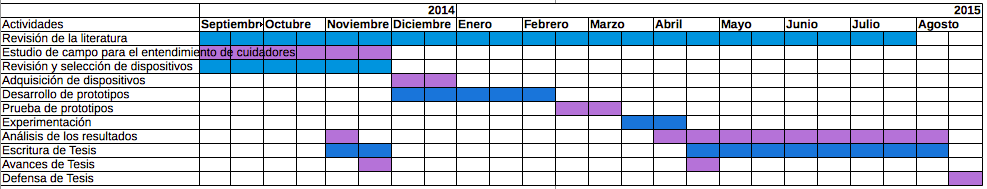
\includegraphics[keepaspectratio=true,scale=.5]{cal.png}
		%	\end{figure}
		%1 StressSense: detecting Stress in Unconstraner Acoustic Environments using smartphones
	%2 A thoerical approach to stress and self-efficacy
	%3 Stress and anxiety, 	Department of Psychophysiological Nursing, School of Nursing, University of Maryland, Baltimore.The Nursing Clinics of North America [1990, 25(4):935-943]
	%4 AutoSense: Unobtrusively Wearable Sensor Suite for Inferring the Onset, Causality, and Consequences of Stress in the Field
	%5
	%6 stress@work
	%7 FEEL: frequent EDA and Event Logging
	\newpage
	\addcontentsline{toc}{chapter}{\normalsize\expandafter{Referencias}}
	{\normalsize
		\bibliographystyle{cicese}
		\bibliography{proposal}
	}
	\end{document}
